\section{Experiments}
\label{sec:experiments}

\subsection{Methodology}
We use the system of \cref{tab:system}.  The 4-core evaluation uses 22 of the 50 mixes, at least four per mix type
and covering every class (homogeneous 1, 3, 5, 7; 2+2: one per class pair; 3+1 and 2+1+1: each class as the majority;
four all-class mixes), at 2.4\,GB/s and 9.6\,GB/s per core.  The 8-core evaluation uses all 20 mixes at 2.4\,GB/s per
core.  The reference is \emph{independent} operation: the native prefetcher on every core and UCP partitioning on its
own.  We report for each design its throughput and harmonic speedup over independent operation, the number of mixes that
lose more than 2\%, the casualties, and the worst core of each mix.  We compare TSC with three prior-style baselines, our own HPAC-style implementations (they are not exact
reproductions of HPAC or CBP):
\begin{itemize}
  \item \textbf{FDT} (fairness-driven throttling, \cref{sec:problem}): under DRAM pressure, trial-throttle the core with
        the most useless (or most) prefetch traffic and keep the step if the fairness score improves; UCP partitions on
        its own.
  \item \textbf{FDT+PSR}: FDT, and the controller owns the partition: starting from the demand-only allocation, cores
        that the prefetch-aware allocation would enlarge receive 80/40/0\% of the extra ways by prefetch-success-rate
        (PSR) tier, taken from donor cores (at most a third of each donor's ways); low-PSR requesters are throttled.
  \item \textbf{FDT+Reclaim}: FDT, and the controller starts from UCP's allocation and reclaims
        $(1-\mathit{PSR}^\gamma)$ of each core's prefetch-won ways, throttling low-PSR requesters in the same trial
        (coupled move), with a victim guard.
\end{itemize}
TSC is evaluated as an ablation, each step adding one component (\cref{tab:suffix}).

\begin{table}[!htbp]
\centering
\caption{TSC variants: each suffix letter adds one component to the previous variant.}
\label{tab:suffix}
\footnotesize
\begin{tabular}{lp{0.68\columnwidth}}
\toprule
Variant & Components \\
\midrule
TSC-T   & \textbf{T}hrottling with throughput-safe acceptance (way-weighted fairness $\uparrow$, throughput $\geq -0.5\%$, throttled
          core $\geq -1\%$), periodic revalidation and the farthest-first prefetch filter; UCP partitions on its own \\
TSC-TP  & + PSR-weighted \textbf{P}artitioning (\cref{sec:method}) \\
TSC-TPG & + \textbf{G}radual re-enabling: own-core test for release trials, step-wise calm release, phase detection \\
TSC     & + accuracy hold with accuracy probes (the full design) \\
\bottomrule
\end{tabular}
\end{table}

\subsection{4-core results}

\begin{table*}[!tp]
\centering
\caption{4-core, 22 mixes per row group: throughput (normalised weighted speedup) and harmonic speedup (HS) vs
independent PF+UCP, the worst mix, the number of mixes losing more than 2\%, casualty cores (independent $\to$
coordinated) and the mean worst core vs neither mechanism (independent $\to$ coordinated).}
\label{tab:final4}
\footnotesize
\begin{tabular}{llcccccc}
\toprule
& Design & Throughput & HS & Worst mix & Mixes $<-2\%$ & Casualties & Worst core \\
\midrule
\multicolumn{8}{l}{\emph{Low bandwidth (2.4 GB/s/core), IPCP, 22 mixes}} \\
& FDT & +5.1\% & +1.3\% & -11.5\% & 5 & 30$\to$26 & 0.78$\to$0.93 \\
& FDT+PSR & +5.1\% & +2.3\% & -16.0\% & 5 & 30$\to$23 & 0.78$\to$0.91 \\
& FDT+Reclaim & +5.8\% & +3.2\% & -11.6\% & 5 & 30$\to$24 & 0.78$\to$0.91 \\
& TSC-T & +4.0\% & +3.4\% & -3.3\% & 2 & 30$\to$28 & 0.78$\to$0.84 \\
& TSC-TP & +3.9\% & +3.4\% & -2.6\% & 1 & 30$\to$28 & 0.78$\to$0.82 \\
& TSC-TPG & +4.6\% & +4.0\% & -2.9\% & 1 & 30$\to$27 & 0.78$\to$0.82 \\
& \textbf{TSC} & +7.1\% & +6.4\% & -2.9\% & 1 & 30$\to$25 & 0.78$\to$0.86 \\
\midrule
\multicolumn{8}{l}{\emph{Low bandwidth (2.4 GB/s/core), Pythia, 22 mixes}} \\
& FDT & -1.3\% & -3.5\% & -9.6\% & 7 & 24$\to$23 & 0.88$\to$0.94 \\
& FDT+PSR & -1.4\% & -2.5\% & -8.7\% & 7 & 24$\to$23 & 0.88$\to$0.91 \\
& FDT+Reclaim & -1.5\% & -2.9\% & -8.7\% & 8 & 24$\to$22 & 0.88$\to$0.91 \\
& TSC-T & +0.3\% & +0.2\% & -2.4\% & 1 & 24$\to$25 & 0.88$\to$0.89 \\
& TSC-TP & +0.2\% & +0.2\% & -0.8\% & 0 & 24$\to$25 & 0.88$\to$0.88 \\
& TSC-TPG & +0.1\% & 0.0\% & -1.2\% & 0 & 24$\to$25 & 0.88$\to$0.89 \\
& \textbf{TSC} & 0.0\% & 0.0\% & -1.2\% & 0 & 24$\to$25 & 0.88$\to$0.89 \\
\midrule
\multicolumn{8}{l}{\emph{Ample bandwidth (9.6 GB/s/core), IPCP, 22 mixes}} \\
& FDT & -0.8\% & -1.0\% & -9.3\% & 4 & 15$\to$13 & 0.96$\to$0.95 \\
& FDT+PSR & -0.9\% & -1.2\% & -16.4\% & 4 & 15$\to$16 & 0.96$\to$0.95 \\
& FDT+Reclaim & -1.2\% & -1.7\% & -14.8\% & 5 & 15$\to$15 & 0.96$\to$0.95 \\
& TSC-T & -0.1\% & -0.1\% & -2.5\% & 1 & 15$\to$13 & 0.96$\to$0.97 \\
& TSC-TP & -0.3\% & -0.4\% & -2.4\% & 1 & 15$\to$15 & 0.96$\to$0.96 \\
& TSC-TPG & 0.0\% & -0.1\% & -2.0\% & 0 & 15$\to$15 & 0.96$\to$0.96 \\
& \textbf{TSC} & +0.6\% & +0.5\% & -2.4\% & 3 & 15$\to$15 & 0.96$\to$0.97 \\
\midrule
\multicolumn{8}{l}{\emph{Ample bandwidth (9.6 GB/s/core), Pythia, 22 mixes}} \\
& FDT & -0.8\% & -0.9\% & -4.7\% & 4 & 8$\to$6 & 1.00$\to$0.99 \\
& FDT+PSR & -1.9\% & -2.2\% & -6.5\% & 6 & 8$\to$11 & 1.00$\to$0.99 \\
& FDT+Reclaim & -1.9\% & -2.2\% & -6.5\% & 8 & 8$\to$11 & 1.00$\to$0.98 \\
& TSC-T & -0.2\% & -0.2\% & -2.2\% & 1 & 8$\to$8 & 1.00$\to$1.00 \\
& TSC-TP & -0.2\% & -0.3\% & -1.4\% & 0 & 8$\to$8 & 1.00$\to$0.99 \\
& TSC-TPG & -0.2\% & -0.2\% & -1.5\% & 0 & 8$\to$8 & 1.00$\to$0.99 \\
& \textbf{TSC} & -0.2\% & -0.2\% & -1.5\% & 0 & 8$\to$8 & 1.00$\to$0.99 \\
\bottomrule
\end{tabular}

\end{table*}

\begin{figure*}[!tp]
\centering
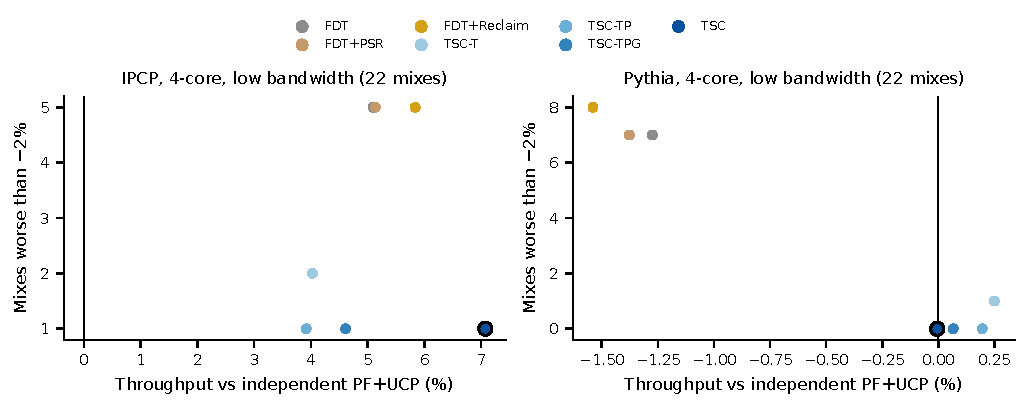
\includegraphics[width=0.9\textwidth]{tradeoff.pdf}
\caption{4-core, 2.4\,GB/s/core: throughput against the number of mixes that lose more than 2\%, for every design
(casualty counts: \cref{tab:final4}).  With IPCP, \vthree{} has the highest throughput and one mix below $-2\%$; with Pythia, all TSC variants are within
0.3\% of independent operation and the prior-style designs lose 1.3--1.5\%.}
\label{fig:tradeoff}
\end{figure*}

\Cref{tab:final4} and \cref{fig:tradeoff} summarise the 4-core results.

\paragraph{Low bandwidth, IPCP}
\vthree{} improves throughput by 7.1\% and harmonic speedup by 6.4\% over independent IPCP+UCP, the best of all
designs, with a single mix below $-2\%$ (worst $-2.9\%$).  The prior-style designs reach 5.1--5.8\% but have five mixes
below $-2\%$ and lose up to 16\%.  \vthree{} reduces the casualties from 30 to 25 and raises the mean worst core from
0.78 to 0.86 of its performance with neither mechanism; the prior-style designs reach 23--26 casualties and
0.91--0.93, with the mix losses above.  In the ablation, the throughput-safe acceptance (TSC-T) reduces the mixes
below $-2\%$ from 5 to 2 at 4.0\% throughput.  Adding the PSR-weighted partition (TSC-TP) changes throughput by
less than 0.2\% (4.0\% $\to$ 3.9\%); gradual re-enabling (TSC-TPG) raises it to 4.6\% and the accuracy hold
(\vthree) to 7.1\%.

\paragraph{Low bandwidth, Pythia}
Every prior-style design loses throughput (1.3--1.5\%, 7--8 mixes below $-2\%$).  \vthree{} causes no regression
(0.0\%, no mix below $-2\%$).  The static oracle finds only \OrcPyMean\% on average with Pythia.  It does not reduce Pythia's casualties (24 $\to$ 25), because these cores are victims of their neighbours'
\emph{useful} prefetching, which TSC largely keeps (see (iii) below).  Three observations from the 24 casualty cores of
the independent run (in 17 of the 22 mixes) support this.  (i)~They are cache-sensitive: 18 are HCLP (low prefetch sensitivity) and 5 HCHP, and their own median prefetch accuracy is only 0.37, against 0.82 over all
cores.  (ii)~Their neighbours prefetch well: the 72 co-running cores have a median accuracy of 0.83, and 60\% of them
run more than 2\% faster with both mechanisms than with neither (median speedup 1.12).  (iii)~Throttling those neighbours
does rescue them, at a net loss: FDT cuts the neighbours' issued prefetches to 37\%, the casualty cores speed up by
9.7\% on average, but the neighbours lose 6.0\% and the mixes 1.3\% of throughput.  TSC keeps 96\% of the
neighbours' prefetches, and both groups stay within 0.7\% of independent operation.  Rescuing the victims of useful
prefetching therefore costs throughput, i.e.\ the benefit of useful prefetchers, which our problem statement rules out.

\paragraph{Ample bandwidth}
At 9.6\,GB/s per core \vthree{} changes throughput by +0.6\% (IPCP) and $-0.2\%$ (Pythia), whereas the prior-style designs lose
0.8--1.9\% with up to eight mixes below $-2\%$ (worst $-16\%$).  Three IPCP mixes lose 2.0--2.4\% under \vthree{} (\cref{sec:limits}).

\begin{figure*}[!tp]
\centering
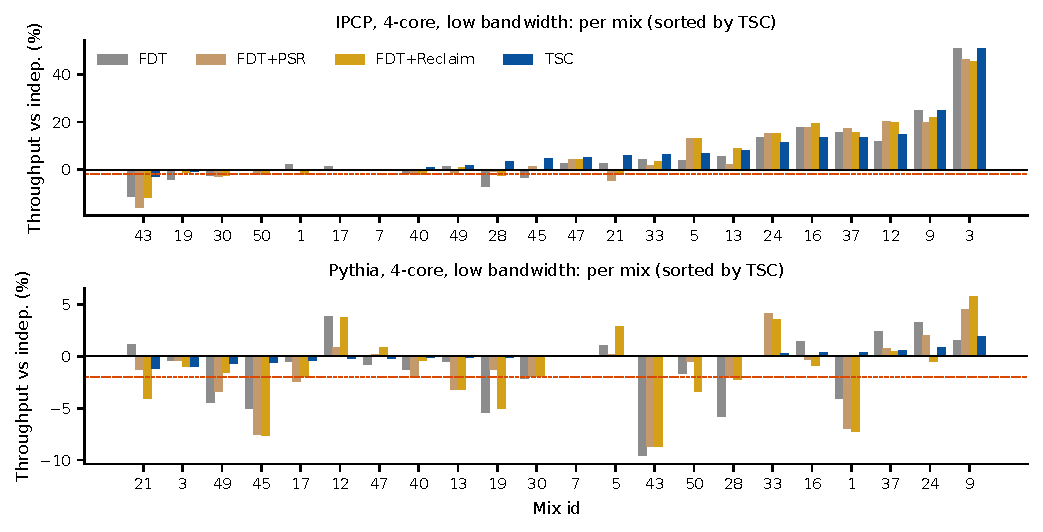
\includegraphics[width=0.9\textwidth]{permix_lowbw.pdf}
\caption{4-core, 2.4\,GB/s/core: per-mix throughput vs independent PF+UCP, sorted by \vthree.  Dashed line: $-2\%$.}
\label{fig:permix}
\end{figure*}

\begin{figure*}[!tp]
\centering
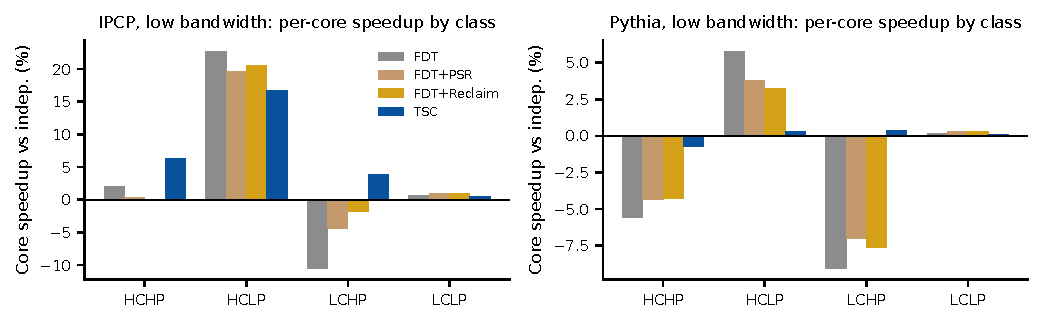
\includegraphics[width=0.9\textwidth]{byclass_lowbw.pdf}
\caption{4-core, 2.4\,GB/s/core: per-core speedup over independent PF+UCP by workload class.}
\label{fig:byclass}
\end{figure*}

\begin{figure*}[!tp]
\centering
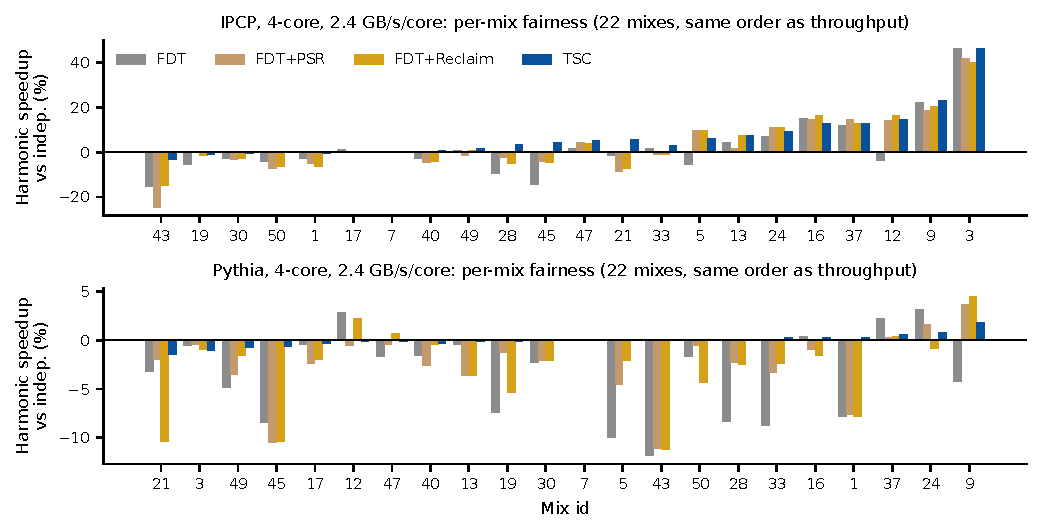
\includegraphics[width=0.9\textwidth]{hs_permix_lowbw.pdf}
\caption{4-core, 2.4\,GB/s/core: per-mix harmonic speedup (fairness) vs independent PF+UCP, mixes in the same order
as \cref{fig:permix}.}
\label{fig:hspermix}
\end{figure*}

\paragraph{Per mix and per class}
\Cref{fig:permix} shows the per-mix results: on the mixes where the prior-style designs gain most (right) \vthree{}
gains as well, and on the mixes where they lose (left) \vthree{} stays within 3\%.  By class (\cref{fig:byclass}), the cache-sensitive, prefetch-insensitive
cores (HCLP) gain the most with IPCP (+17\%); unlike FDT, \vthree{} does not sacrifice the LCHP cores,
whose prefetchers are useful ($-10\%$ under FDT, +4\% under \vthree).  \Cref{fig:hspermix} shows the same mixes for fairness: \vthree{} raises the harmonic speedup by more than 2\% in 13
of 22 IPCP mixes and lowers it by more than 2\% in one (worst $-3.0\%$), whereas the prior-style designs lower it by
more than 2\% in 8--10 IPCP and 11--12 Pythia mixes (worst $-24.8\%$).  With Pythia, \vthree{} stays within 2\% of
independent operation in every mix.

\subsection{8-core results}

\begin{table*}[!tp]
\centering
\caption{8-core, 2.4\,GB/s/core (columns as in \cref{tab:final4}).  All designs are compared on the mixes for which
\vthree{} has finished.}
\label{tab:eight}
\footnotesize
\begin{tabular}{llcccccc}
\toprule
& Design & Throughput & HS & Worst mix & Mixes $<-2\%$ & Casualties & Worst core \\
\midrule
\multicolumn{8}{l}{\emph{8-core, 2.4 GB/s/core, IPCP, 19 of 20 mixes (mix 05 pending)}} \\
& FDT & +7.4\% & +3.2\% & -7.9\% & 2 & 53$\to$49 & 0.70$\to$0.88 \\
& FDT+PSR & +3.6\% & +0.6\% & -13.8\% & 8 & 53$\to$57 & 0.70$\to$0.80 \\
& FDT+Reclaim & +4.3\% & +1.3\% & -7.6\% & 7 & 53$\to$55 & 0.70$\to$0.79 \\
& \textbf{TSC} & +6.0\% & +5.2\% & -1.2\% & 0 & 53$\to$48 & 0.70$\to$0.75 \\
\midrule
\multicolumn{8}{l}{\emph{8-core, 2.4 GB/s/core, Pythia, 19 of 20 mixes (mix 05 pending)}} \\
& FDT & -2.2\% & -5.4\% & -15.7\% & 8 & 37$\to$41 & 0.79$\to$0.89 \\
& FDT+PSR & -3.8\% & -5.8\% & -21.0\% & 9 & 37$\to$45 & 0.79$\to$0.82 \\
& FDT+Reclaim & -3.1\% & -4.8\% & -12.8\% & 12 & 37$\to$41 & 0.79$\to$0.83 \\
& \textbf{TSC} & +0.1\% & 0.0\% & -0.7\% & 0 & 37$\to$37 & 0.79$\to$0.79 \\
\bottomrule
\end{tabular}

\end{table*}

\Cref{tab:eight} compares the designs on the 19 of 20 8-core mixes for which \vthree{} has finished (mix 05 is still
running).

\paragraph{IPCP}
\vthree{} improves throughput by 6.0\% and harmonic speedup by 5.2\% with no mix below $-2\%$ (worst mix $-1.2\%$).
FDT reaches a higher throughput (7.4\%) but has two mixes below $-2\%$ (worst $-7.9\%$); FDT+PSR and FDT+Reclaim reach
3.6--4.3\% with 7--8 such mixes (worst $-13.8\%$).  \vthree{} has the highest harmonic speedup and the fewest
casualties (53 $\to$ 48, FDT 49), while FDT raises the mean worst core more (0.70 $\to$ 0.88, \vthree{} 0.75).

\paragraph{Pythia}
\vthree{} changes throughput by $+0.1\%$ with no mix below $-2\%$ (worst $-0.7\%$) and leaves the casualties
unchanged (37).  Every prior-style design loses throughput (2.2--3.8\%), has 8--12 mixes below $-2\%$ (worst
$-21.0\%$) and raises the casualties to 41--45.

\begin{figure*}[!tp]
\centering
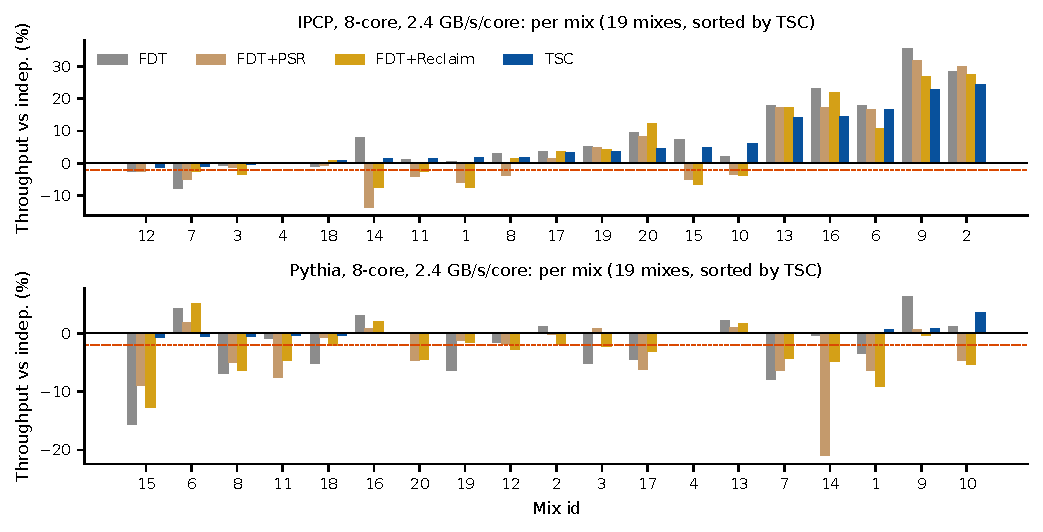
\includegraphics[width=0.9\textwidth]{permix_8core.pdf}
\caption{8-core, 2.4\,GB/s/core: per-mix throughput vs independent PF+UCP, sorted by \vthree{}, on the mixes for
which every design has finished.  Dashed line: $-2\%$.}
\label{fig:permix8}
\end{figure*}

\begin{figure*}[!tp]
\centering
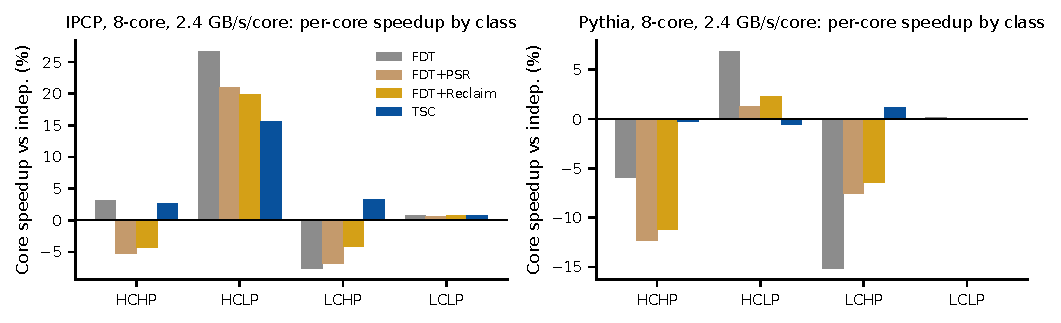
\includegraphics[width=0.9\textwidth]{byclass_8core_designs.pdf}
\caption{8-core, 2.4\,GB/s/core: per-core speedup over independent PF+UCP by workload class, on the same mixes as
\cref{fig:permix8}.}
\label{fig:byclass8}
\end{figure*}

\begin{figure*}[!tp]
\centering
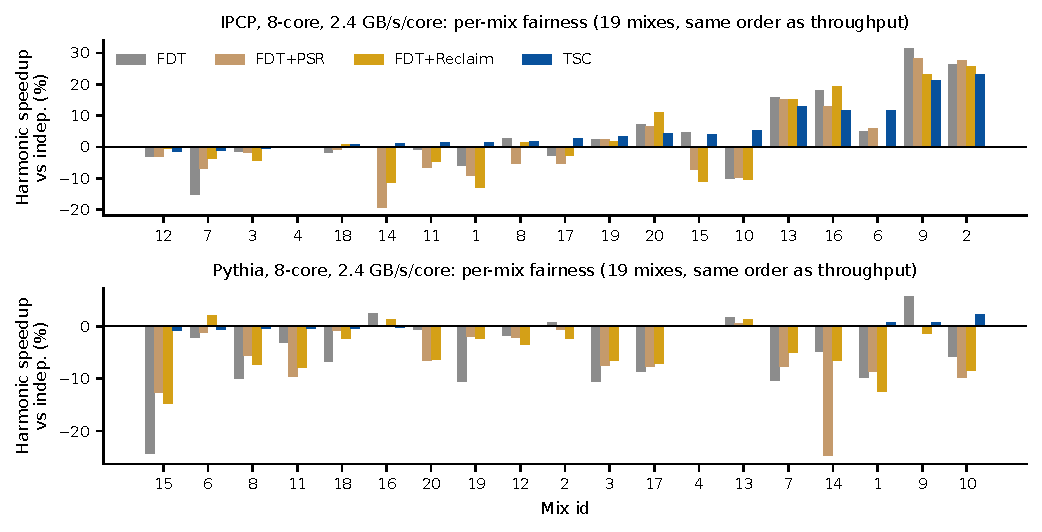
\includegraphics[width=0.9\textwidth]{hs_permix_8core.pdf}
\caption{8-core, 2.4\,GB/s/core: per-mix harmonic speedup (fairness) vs independent PF+UCP, mixes in the same order as
\cref{fig:permix8}.}
\label{fig:hspermix8}
\end{figure*}

\Cref{fig:permix8,fig:hspermix8,fig:byclass8} show the 8-core results per mix (throughput and fairness) and per
workload class.

\subsection{Sensitivity}
\label{sec:sweep}

\begin{table}[!htbp]
\centering
\caption{Sensitivity of \vthree{}, 4-core, 2.4\,GB/s/core: throughput change relative to \vthree{} with default
parameters on the same mixes, one parameter changed at a time.}
\label{tab:sweep}
\footnotesize
\begin{tabular}{lcrcc}
\toprule
Parameter (default) & Value & Mixes & IPCP & Pythia \\
\midrule
Accuracy hold (0.15) & 0.10 & 10 & -1.3\% & -0.2\% \\
Accuracy hold (0.15) & 0.20 & 10 & +0.5\% & -0.1\% \\
Own-core budget (1\%) & 3\% & 22 & -0.1\% & +0.0\% \\
\bottomrule
\end{tabular}

\end{table}

\Cref{tab:sweep} varies the parameters that only \vthree{} has, one at a time.  Raising the accuracy hold from 0.15 to 0.20 changes IPCP throughput by $+0.5\%$, lowering it to 0.10 by
$-1.3\%$; Pythia changes by at most 0.2\%.  Relaxing the own-core budget from 1\% to 3\% changes throughput by at
most 0.1\%.  The
mechanisms that \vthree{} shares with the prior-style designs (two-level drop, victim guard, partition step) were
swept on FDT+Reclaim during the design; there, only disabling the two-level drop, a 5\% victim guard and a one-way
partition step cost more than 1\%, so we kept their reference values.

\subsection{Limitations}
\label{sec:limits}
\begin{itemize}
  \item \textbf{Ample bandwidth.}  In the three IPCP mixes that lose 2.0--2.4\% at 9.6\,GB/s per core, single cores
        lose 4.5--8.4\%.  In mix 49 a core with accuracy 0.05 is held at level 1 for 441 of 466 epochs and loses
        8.4\%, although with both mechanisms it runs 6.5\% faster than with neither; in mix 12 a core with accuracy
        0.07 loses 6.6\%; in mix 1 two cores with accuracy 0.19 and 0.32 are throttled in 17--18\% of the epochs and
        lose 4.5\% and 6.3\%.  Letting a calm DRAM release held cores as well is one option we have not evaluated.
  \item \textbf{Static headroom at ample bandwidth.}  At 9.6\,GB/s per core the static oracle finds \OrcIpMean\% for
        IPCP (on its \OrcIpN{} mixes), whereas \vthree{} gains 0.6\% (on 22 mixes).  \vthree{} throttles only when
        DRAM is busy; whether an own-core test that runs also when DRAM is calm captures this headroom is open.
  \item \textbf{Victims of useful prefetching} are not rescued (Pythia, \cref{sec:experiments}).
  \item \textbf{Measurement noise}: decisions rest on two-epoch IPC measurements.
  \item \textbf{Context switches} do not occur in our trace-driven runs; on a real system a core's level and
        statistics would be reset on a context switch.
\end{itemize}
